\section{Related Work}
\label{section:bgrelated}

Whilst session type theory represents 
the type language for concurrent processes,
it also forms the theoretical basis for proposals
introduced to implement session types for 
real-world application development:
the \textit{Scribble} project is one such proposal.
We discuss related work that 
implement session types for software
engineering using the Scribble project
in \cref{subsection:bgscribble},
and focus on existing work for
session-typed web development
in \cref{subsection:sessiontypewebdev}.

\subsection{Scribble and Endpoint API Generation}
\label{subsection:bgscribble}

% Introduce Scribble as an implementation of MPST
Scribble \cite{Scribble} is a
platform-independent description language 
for the specification of message-passing protocols.
The language describes the behaviour of 
communicating processes at a high level of abstraction:
more importantly, the description is independent from 
implementation details in the same way that 
the type signature of a function declaration is decoupled 
from the corresponding function definition.

A Scribble \textit{protocol specification} 
describes an agreement of how participating systems, 
referred to as \text{roles}, interact. 
The protocol stipulates the sequence of structured messages 
exchanged between roles; 
each message is labelled with a name and the
type of payload carried by the message.

We present an example of a Scribble protocol in 
\cref{fig:adder} adapted from \cite{Hybrid2016}.
The protocol specifies an arithmetic web service 
offered by a \trole{S}erver to a \trole{C}lient.
The \trole{C}lient is permitted to either:

\begin{itemize}
\item 
Send two \texttt{int}s attached to an \tmsg{Add} message, 
where the server will respond with an \texttt{int} in a 
message labelled \tmsg{Res}, and the protocol restarts; or,
\item
Send a \tmsg{Quit} message, where the server will 
respond with a \tmsg{Terminate} message and the protocol ends.
\end{itemize}

\begin{figure}[!ht]
\begin{lstlisting}[language=Scribble]
type <java> "java.lang.Integer" from "rt.jar" as int; (*@\label{line:typedecl}@*)

global protocol Adder(role C, role S) {
	choice at C {
		Add(int, int)	from C to S;
		Res(int)		from S to C;
		do Adder(C, S);
	} or {
		Quit()		from C to S;
		Terminate()	from S to C;	
	}
}
\end{lstlisting}
\caption{Adder Protocol in Scribble}
\label{fig:adder}
\end{figure}

The platform-independent nature of Scribble 
can be observed from the \texttt{type} declaration 
on \cref{line:typedecl}: 
the developer has the freedom to specify message payload formats 
and data types from the target language of the implementation 
-- in this case, aliasing the built-in Java integer as 
\texttt{int} throughout the protocol.

To observe the parallels between MPST theory
and the Scribble language,
we present the corresponding global type for
the \tprotocol{Adder} protocol below.

\[
G_\text{Adder} = \trec{
\gcommone{C}{S}{
	\begin{cases}
		\tmsg{Add(int, int)} & :
			\gcommone{S}{C}{\tmsg{Res(int)}}. ~\trecvar \\
		\tmsg{Quit()} & : 
			\gcommone{S}{C}{\tmsg{Terminate()}}.~ \tend \\		
	\end{cases}
}} 
\]

The protocol specification language is 
a component of the broader 
\textit{Scribble toolchain} initiated by 
Honda et al. \cite{Scribble}, 
through which the toolchain also facilitates 
the development of 
\textit{endpoint applications} that 
conform to user-specified protocols.

A Scribble global protocol can be projected
to a role, or \textit{endpoint},
to obtain a \textit{local protocol} 
which represents
the global protocol viewed from the perspective
of the endpoint.
This allows the endpoint to \textit{verify} their
implementation against their local protocol
for conformance, independent of other endpoints.
The communication safety guarantees from MPST
theory also apply here: if the implementation
for each endpoint is verified against their
local protocol, the distributed system as
a whole will conform to the global protocol.

The Scribble toolchain can convert the local
protocol into an \textit{endpoint finite state machine}
(EFSM).
An EFSM encodes the control flow of the local
protocol into a communication automaton:
there is a well-defined initial \textit{state},
and each \textit{transition} from some state to a
successor state corresponds to a valid communication
action (i.e. sending or receiving a message) permitted
at that endpoint at that state.

\begin{figure}[!h]
\centering
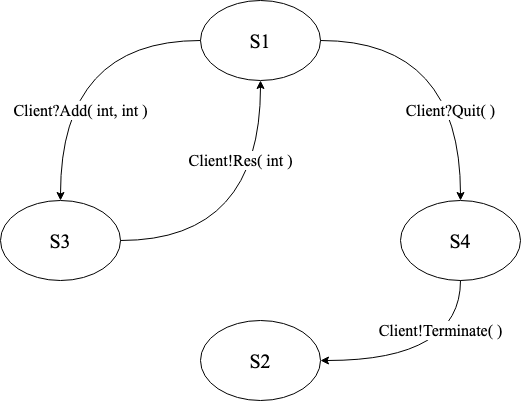
\includegraphics[width=.7\textwidth]{BGAdderFSM}
\captionof{figure}{Server EFSM for Adder protocol}
\label{fig:bgadderfsm}
\end{figure}

We show the EFSM of the \trole{Server} for the
\tprotocol{Adder} protocol in \cref{fig:bgadderfsm}.
We use this as an example to walk through
the components that build up the EFSM.

\begin{itemize}

\item \textbf{Role Identifiers:}
The set of roles that the endpoint interacts with.
For \cref{fig:bgadderfsm}, this is the singleton set
$\{~\trole{Client}~\}$.

\item \textbf{Label Identifiers:}
The set of message labels that the endpoint sends or
expects to receive.
For \cref{fig:bgadderfsm}, this is set
$\{~\tmsg{Add}, \tmsg{Res}, \tmsg{Quit}, \tmsg{Terminate}~\}$.

\item \textbf{Payload Types:}
The set of message payload data types that the endpoint
sends or expects to receive.
For \cref{fig:bgadderfsm}, this is singleton set
$\{~\texttt{int}~\}$.

\item \textbf{Actions:}
The set of send and receive actions permitted for the endpoint.
An action is defined in terms of a role identifier,
label identifier and a vector of payload types.
For \cref{fig:bgadderfsm}, this is the set of visible
transitions as illustrated.

$\texttt{Client!Terminate()}$ denotes a \textit{send action}
that sends the \tmsg{Terminate} message with 
no payload to \trole{Client}.

$\texttt{Client?Add(int,int)}$ denotes a \textit{receive action}
that receives the \tmsg{Add} message with two \texttt{int}
values as payload from \trole{Client}.

\item \textbf{State Identifiers:}
For \cref{fig:bgadderfsm}, this is the set 
$\{~ \tmsg{S1}, \tmsg{S2}, \tmsg{S3}, \tmsg{S4}~\}$.

\item \textbf{State Transition Function:}
The \textit{partial function}, denoted $\delta$ in the literature,
which maps state identifiers and actions to
successor state identifiers.
It is a partial function because not all tuples
of state identifiers and actions constitute valid transitions
permitted in the state machine.

For \cref{fig:bgadderfsm},
(\texttt{S1, Client?Add(int,int)}) is in the domain
of $\delta$; the successor state is \texttt{S3}.
Conversely, $\delta($\texttt{S1, Client!Res(int)}$)$
is undefined.
\end{itemize}

We also inherit the characteristics of EFSMs derived
from well-formed protocols, as presented in \cite{Hybrid2016}:

\begin{itemize}
\item 
There is \textit{exactly one} initial state 
(\texttt{S1} in \cref{fig:bgadderfsm}).

An initial state has no incoming transitions.
Formally, the state identifier of the initial state
is not in the range of $\delta$.

\item 
There is \textit{at most one} terminal state 
(\texttt{S2} in \cref{fig:bgadderfsm}).

A terminal state has no outgoing transitions.
Formally, the state identifier of the terminal state
is not in the domain of $\delta$.

\item
Every non-terminal state is either a \textit{send}
state or a \textit{receive} state.

A send state only has send actions in its
outgoing transitions. \texttt{S3} and \texttt{S4}
are the send states in \cref{fig:bgadderfsm}.

A receive state only has receive actions in its
outgoing transitions. \texttt{S1} is the only
receive state in \cref{fig:bgadderfsm}.
\end{itemize}

Developers can use the EFSM to verify their implementation
for protocol conformance with respect to an endpoint
in the global protocol.
Endpoint API generation is a common approach
\cite{HuJava,Hybrid2016,Python2017,PureScript2019,LinearDecomp}:
these proposals generate APIs in the target language
which the developer
can use to implement their endpoint application
and enjoy the following guarantees:

\begin{itemize}

\item \textbf{Behavioural typing:}
The execution trace of messages sent and received by
the application is accepted by the EFSM, which means it
conforms to the communication structure of the global protocol;

\item \textbf{Channel linearity:}
Each transition in the EFSM represents one channel resource.
The application transitions from some state $S$
to some successor state $S'$
once \textit{and only once},
after which it must no longer
be able to access a reference (e.g. have an alias) to $S$.
\end{itemize}

We highlight two distinct proposals for endpoint
API generation that differ
by how they leverage features in the target language
to guarantee the above properties.

\subsubsection{Hybrid Session Verification in Java \cite{Hybrid2016}}
Hu and Yoshida implemented a workflow
that performs \textit{hybrid} verification of 
communication protocol conformance for Java applications.
The ``hybrid'' concept is composed of the two main components below:

\subparagraph{Static session typing}
The EFSM is interpreted under the object-oriented paradigm as follow:
\textbf{(1)} states are represented as classes;
\textbf{(2)} supported transitions on each state are 
represented as instance methods,
parameterised by the role, label and payload involved 
in the message exchange. 
A send method takes the payload to send as a parameter,
whilst a receive method is a blocking call that 
requires the caller to allocate a \texttt{Buf<T>} wrapper 
on the stack (where \texttt{T} is the expected payload type),
then the receive method populates the payload into 
the wrapper and returns upon receiving from the channel. 
These instance methods return a new instance of 
the successor state class.

\subparagraph{Runtime channel linearity checks}
By exposing send and receive actions as instance
methods, the developer can keep aliases of EFSM state instances
and invoke the IO action more than once. Java does not
have a linear type system, and hence cannot statically
verify linear usage; this means linearity checks need to be
done at runtime.
Each state keeps track of its usage in a private boolean flag 
and throws an exception when the instance method is called twice.
Similarly, the \texttt{SessionEndpoint} class keeps track of 
whether the connection is open or close,
and throws an exception when program execution exits the 
scope of the session endpoint and a terminal state 
has yet to be reached.\\

We find that this proposal strikes a good balance 
between maximising static communication safety guarantees 
whilst providing an intuitive set of APIs for developers 
to efficiently write their applications. 
For example, the EFSM encoding takes advantage of the type system 
to statically enforce valid transitions; whilst this
exposes channel resources and linear usage needs to be
monitored dynamically to compensate for the lack of linear types,
the generated APIs complement the 
imperative style of application code written in Java


\subsubsection{Runtime Monitors in Python \cite{Python2017} }
Neykova targeted the MPST methodology 
for Python programs
and proposed to generate \textit{runtime monitors} 
from the EFSM.
These monitors expose APIs for sending and receiving messages,
which is used by the developer in their implementation. 
The runtime monitor is an abstraction between the 
developer's implementation and the actual communication channel, 
and ``executes'' the EFSM internally to ensure protocol conformance. 
When the developer sends a message (with some label and payload) 
using the API, the runtime monitor checks 
whether this send action conforms to the current EFSM state, 
and if so, 
performs the send and advances to the successor state. 
Likewise, when the developer invokes a receive, 
the runtime monitor verifies that this is permitted 
at the current EFSM state before returning the received payload.

We observe that this approach complements the 
dynamic typing nature of the Python language, 
which makes it sensible to perform behavioural typing at runtime.
As the send and receive IO primitives are
made available to the developer,
there are no ``instances'' of channel resources created,
so the developer cannot explicitly hold a reference to
some state in the EFSM (let alone keep aliases),
so channel linearity is trivially guaranteed here.

\subsection{Session Types in Web Development}
\label{subsection:sessiontypewebdev}

We discuss the current state-of-the-art proposals
for session-typed web development.

\subsubsection{API Generation in PureScript \cite{PureScript2019}}
King et al. presented an approach
for integrating \textit{multiparty} session types 
into web development using 
the PureScript language \cite{PureScript}.
PureScript is a strongly typed functional language
that compiles to JavaScript.
This proposal takes advantage of its expressive type system to 
provide \textit{static} guarantees for protocol conformance.
We outline the main components of their EFSM encoding:

\subparagraph{Actions as type classes} 
The semantics of the state transition function 
in the EFSM express that a \texttt{(state, action)} tuple
\textit{uniquely defines} a successor \texttt{state}. 
These semantics can be expressed by 
\textit{multi-parameter type classes (MPTC) 
with functional dependencies}: 
\lstonelineps{class Send r s t a | s -> t r a} 
defines \texttt{Send} as a MPTC 
parameterised by recipient \texttt{r}, 
current state \texttt{s}, successor state \texttt{t} 
and payload type \texttt{a}; 
\texttt{s -> t r a} expresses the functional dependency that, 
for an instance of this type class, 
the current state uniquely determines the
successor state, the recipient and payload type. 
These type classes are independent of the EFSM.

\subparagraph{Transitions as instances of type classes} 
By encoding states as data types, 
valid EFSM transitions are encoded as 
\textit{instances} of the type classes. 
If \texttt{S1} is an output state, 
sending an \texttt{Int} to \texttt{Svr} with 
successor state \texttt{S2}, the PureScript encoding would be
\lstonelineps{instance SendS1 :: Send Svr S1 S2 Int}.
Because of the functional dependency, 
the developer cannot instantiate an invalid transition 
(e.g. \lstonelineps{Send Svr S1 S3 Bool}, 
since \texttt{S1} uniquely determines the other type parameters. 
PureScript statically resolves these type constraints at
compile time.

\subparagraph{Channel linearity by construction}
Whilst PureScript does not support linear types,
this proposal carefully designed the session runtime using 
a collection of communication combinators to conceal the
channel resource, which guarantees channel linearity by construction.\\

This proposal is relevant to the problem we are tackling.
In particular, the final point about guaranteeing channel linearity
by construction is something we can build upon in our solution,
since linear types is a feature left to be desired in
``mainstream'' programming languages.
We also observe the challenges of session-typed GUI
programming, as shown by the careful choice 
made in \cite{PureScript2019} 
to use the \textit{Concur UI} framework \cite{ConcurUI} which 
builds UI elements sequentially to model sequential sessions.
Not doing so would make channel linearity violation possible 
(e.g. by binding a send transition to a button click event,
the button may still be active after the transition is complete;
clicking on it again will reuse the channel resource).
Whilst King et al. \cite{PureScript2019} supports 
multiparty session types,
the communication protocol must describe all interactions
to go through a centralised server role to respect the
network topology enforced by WebSocket transport.

As motivated in \cref{section:intro}, 
the functional paradigm and sequential UI framework
are necessary features for the proposal to statically 
provide communication safety guarantees, but 
this type of workflow is not compatible with 
modern web programming practices and compromises on usability.

\subsubsection{Session-Typed GUI Programming 
using Links \cite{MVU2020}}
Fowler presented the first formal integration
of session typing and GUI programming.
His work formalised the \textit{Model-View-Update} (MVU)
architectural pattern for GUI development.
An MVU application features a \textit{model} encapsulating application
state, a \textit{view function} rendering the state on the 
user interface, and an
\textit{update function} handling
\textit{messages} produced by the
rendered model to produce a new model.
Fowler introduces the concept of model types
to express type dependencies between these components:
a \emph{model type} uniquely defines a \textit{view} function,
set of \textit{messages} and \textit{update function} --
rather than producing a new model, the update function 
defines valid transitions to other model types.
This approach guarantees channel linearity for GUI programming:
the update function transitions to a successor model, which only
renders an interface with the set of messages unique to that model,
so channel actions from the predecessor model are not rendered,
which makes reuse impossible.
The core MVU calculus is also extended with \textit{commands}
and \textit{linearity} required to express communication
actions in session type theory.

Fowler's proposal \cite{MVU2020} is implemented using
the \textit{Links} web programming language
\cite{LINKS}. Links is a strict, typed, functional language
that can be used to write full-stack web applications;
and similar to PureScript, it is compiled to JavaScript.
As it has a linear type system, session types can be
implemented using native language features to
monitor linear channel usage.
Links also supports error handling for session types,
as introduced in \cite{Exceptional}; 
given side-effects must be made explicit
in functional programming,
Fowler et al. \cite{Exceptional} introduces
a \textit{session cancellation} operator to ensure
that channel resources are closed after handling
side-effects, such as errors.

This work succeeds in 
retaining the declarative approach for writing
web interfaces, as the view function incorporates standard
\textit{Hyper-Text Mark-up Language} (HTML).
The novel approach of guaranteeing channel linearity
in GUI programming through the model type abstraction
is something we can build upon. 
However, Links does not support multiparty session types,
and similar to \cite{PureScript2019},
it can only express server-centric communication structures
over WebSocket transport.